% English version of paper/ja_v2/07_総合考察.md (2026-11-17).
\section{Discussion}\label{sec:discussion}

\subsection{From the analysis to the method}
The answers to RQ1(a) and RQ1(b) set the next question and the design of the proposal (Fig.~\ref{fig:story}). RQ1(a) showed that, with one source corpus, audio and visual answer bias was almost removed without labels, and that, with all other corpora as sources, the remaining error was reduced by pseudo-labels from classifiers including other modalities, so RQ1(b) focused on distillation. RQ1(b) showed that distillation raised the point estimate of audio UAR, that in post hoc variants at K = 5 and 25 UAR rose only with pseudo-labels of higher UAR than the retrained classifier (Sect.~\ref{sec:rq1b-margin}), and that the strongest modality differed by corpus. RQ2 therefore combined predictions with weights per classifier and emotion, taking only three strengths from the few K labels, profiles from the sources and hyperparameters from source-corpus episodes.

\begin{figure}[t]
\centering
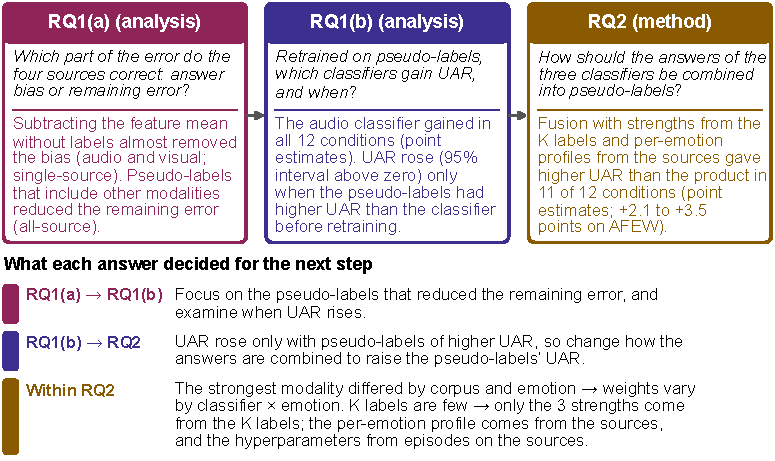
\includegraphics[width=\textwidth]{figures/fig_story_en.pdf}
\caption{How the three questions and their answers connect. Top: each question and its answer. Bottom: what each answer decided for the next step}\label{fig:story}
\end{figure}

\subsection{What this study adds to prior work}
Albanie et al.\ \cite{albanie2018} showed that audio classifiers can be trained on facial predictions, and training on predictions of a more accurate model of another modality has been reported not to always help \cite{xue2023mfh}; we found, in cross-corpus MER on four corpora with a few target labels, that in post hoc variants at K = 5 and 25 UAR rose only when the pseudo-labels had higher UAR than the classifier before retraining. Whereas domain adaptation studies compared methods that combine information sources \cite{ganin2016dann,saito2019mme}, we measured which part of the error each source corrects, and for the audio classifier, 11 methods without pseudo-labels including other modalities had lower UAR than distillation in point estimates. Busso et al.\ \cite{busso2004} found modality strengths to differ by emotion within one corpus, and Kaya et al.\ \cite{kaya2017} chose model-by-emotion weights by random search on labelled validation data. We found that the strongest modality also changed across our corpora and, with only K labels per emotion, measured strengths on the K labels, per-emotion profiles on the sources and hyperparameters on source-corpus episodes, so that emotion-wise weights can be set with a few target labels. Unlike Ryumina et al.\ \cite{ryumina2025}, who used no target labels, we used a few target labels and unlabelled target utterances.

\subsection{Where to spend effort on a new corpus}
The results inform whether to spend effort on labelling or on collecting unlabelled recordings for a new corpus. First, the audio classifier retrained on unlabelled utterances and pseudo-labels alone (K = 0) had higher UAR in point estimates (no intervals computed) than the K-label baselines with 5 and 10 labels per emotion on all four corpora (Sect.~\ref{sec:rq1b-audio}). Second, when the pseudo-labels had lower UAR than the classifier before retraining, UAR did not rise (Sect.~\ref{sec:rq1b-margin}). Third, a few labels were useful for measuring classifier strengths when combining predictions (Sect.~\ref{sec:rq2-results}). These results suggest, for a new corpus, collecting unlabelled multimodal recordings for distillation and using the few labels to measure classifier strengths.
